\documentclass[a4paper]{article}
%\usepackage{luacode}

% Graphical Packages
\usepackage[margin=2cm,includeheadfoot, nomarginpar,]{geometry}
\usepackage{graphicx, fancyhdr, setspace}
\usepackage{tikz, tcolorbox}
\usetikzlibrary{shapes, shadows}

% Maths Packages
\usepackage{amsmath, amsfonts, amsthm}

% Formatting Packages
\usepackage{fontspec, titlesec}
\usepackage[automake, acronym]{glossaries-extra}
\usepackage{authblk, hyperref, float, array, multirow, colortbl}
\usepackage{color, xcolor}
\usepackage{listings, listings-rust}

% Glossary
\setabbreviationstyle[acronym]{long-short}
\newacronym{ex}{ex.}{example} %Creates an acronym for 'example', the writer will type 'ex', the displayed version will be 'ex.'
% Other acronyms
\makeglossaries

% Bibliography
\usepackage[style=apa, parentracker=true]{biblatex}
\addbibresource{myLibrary.bib}

% Colour Defining
\definecolor{codebg}{rgb}{0.11,0.12,0.13} % Dark background
\definecolor{codebasic}{rgb}{0.73,0.74,0.76} % Dark background
\definecolor{codecomment}{rgb}{0.44,0.45,0.47} % Gray for comments
\definecolor{codestring}{rgb}{0.41,0.60,0.31} % Green for strings
\definecolor{codekey1}{rgb}{0.97,0.33,0.39} % Red for keywords
\definecolor{codekey2}{rgb}{0.20,0.13,0.79} % Red for keywords

% Code Snippets Styling
% Note: Might want to swap listings for fancyvbr package
\renewcommand\lstlistingname{Source Code}
\renewcommand\lstlistlistingname{Source Code}
\lstdefinestyle{mystyle}{
	language=Rust, 
	backgroundcolor=\color{codebg},
	basicstyle=\ttfamily\footnotesize\color{codebasic},
	commentstyle=\color{codecomment}, 
	stringstyle=\color{codestring},
	keywordstyle=\bfseries,% reserved keywords
	%keywordstyle=[2]\color{codekey2},% traits
	%keywordstyle=[3]\color{codekey2},% primitive types
	%keywordstyle=[4]\color{codekey2},% type and value constructors
	keywordstyle=[5]\color{codekey1},% macros
	%
	breaklines=true,
	breakatwhitespace=true, 
	numbers=left,
	firstnumber=auto,
	numbersep=5pt,
	tabsize=4,
	xleftmargin=10pt,
	showstringspaces=false,
	showspaces=false,
	showtabs=false,
	columns=spaceflexible,
	keepspaces=true,
	frame=left,
	framesep=5pt,
	framerule=10pt,
	rulecolor=\color[gray]{0.30},
	mathescape=true,
	captionpos=b,
}

% Page Styling
\usepackage{lipsum} % Dummy text for demonstration
\pagestyle{fancy}

% Table Styling
\setlength{\tabcolsep}{18pt} % Gap before text
\renewcommand{\arraystretch}{1.5} % Cell height scaling
\setlength{\arrayrulewidth}{0.5mm} % Thickness of the table borders
% \arrayrulecolor{blue}		%set border colour. Requires package [table]{xcolor} 

% Font Styling
\setmainfont{JetBrainsMono NF Medium}
\newfontfamily\sectionfont{JetBrainsMono NF Bold}

\titleformat{\section}
{\sectionfont\bfseries\Large} % Bold and large font for sections
{\thesection.}    % Section number (optional)
{1em}             % Spacing between number and title
{\_}

% Header & Footer Styling
\lhead{Marco Ramos}
\rhead{Student ID: 10415201}
\cfoot{
\includegraphics[width=1cm]{img/coventry-phoenix.png}}
\rfoot{> Page \thepage\ <}
\onehalfspacing

% Hyperlink Styling
\hypersetup{
	colorlinks=true,
	linkcolor=blue, % Internal link colour
	urlcolor=red, % External link colour
	pdftitle={LaTeX Template}, % Title to display in PDF Readers
	}


% Document Info
\title{\LaTeX\ Template}
\author[1]{Marco Ramos}
\affil[1]{Coventry University, Coventry, UK}


\begin{document}
	% COVER PAGE
	\newgeometry{margin=0pt} % Set zero margins for the first page
\thispagestyle{empty} % Remove page number and header/footer for the first page


\hspace*{-0.61cm} %shift left
\vspace*{-1cm} %allow negative y coordinates
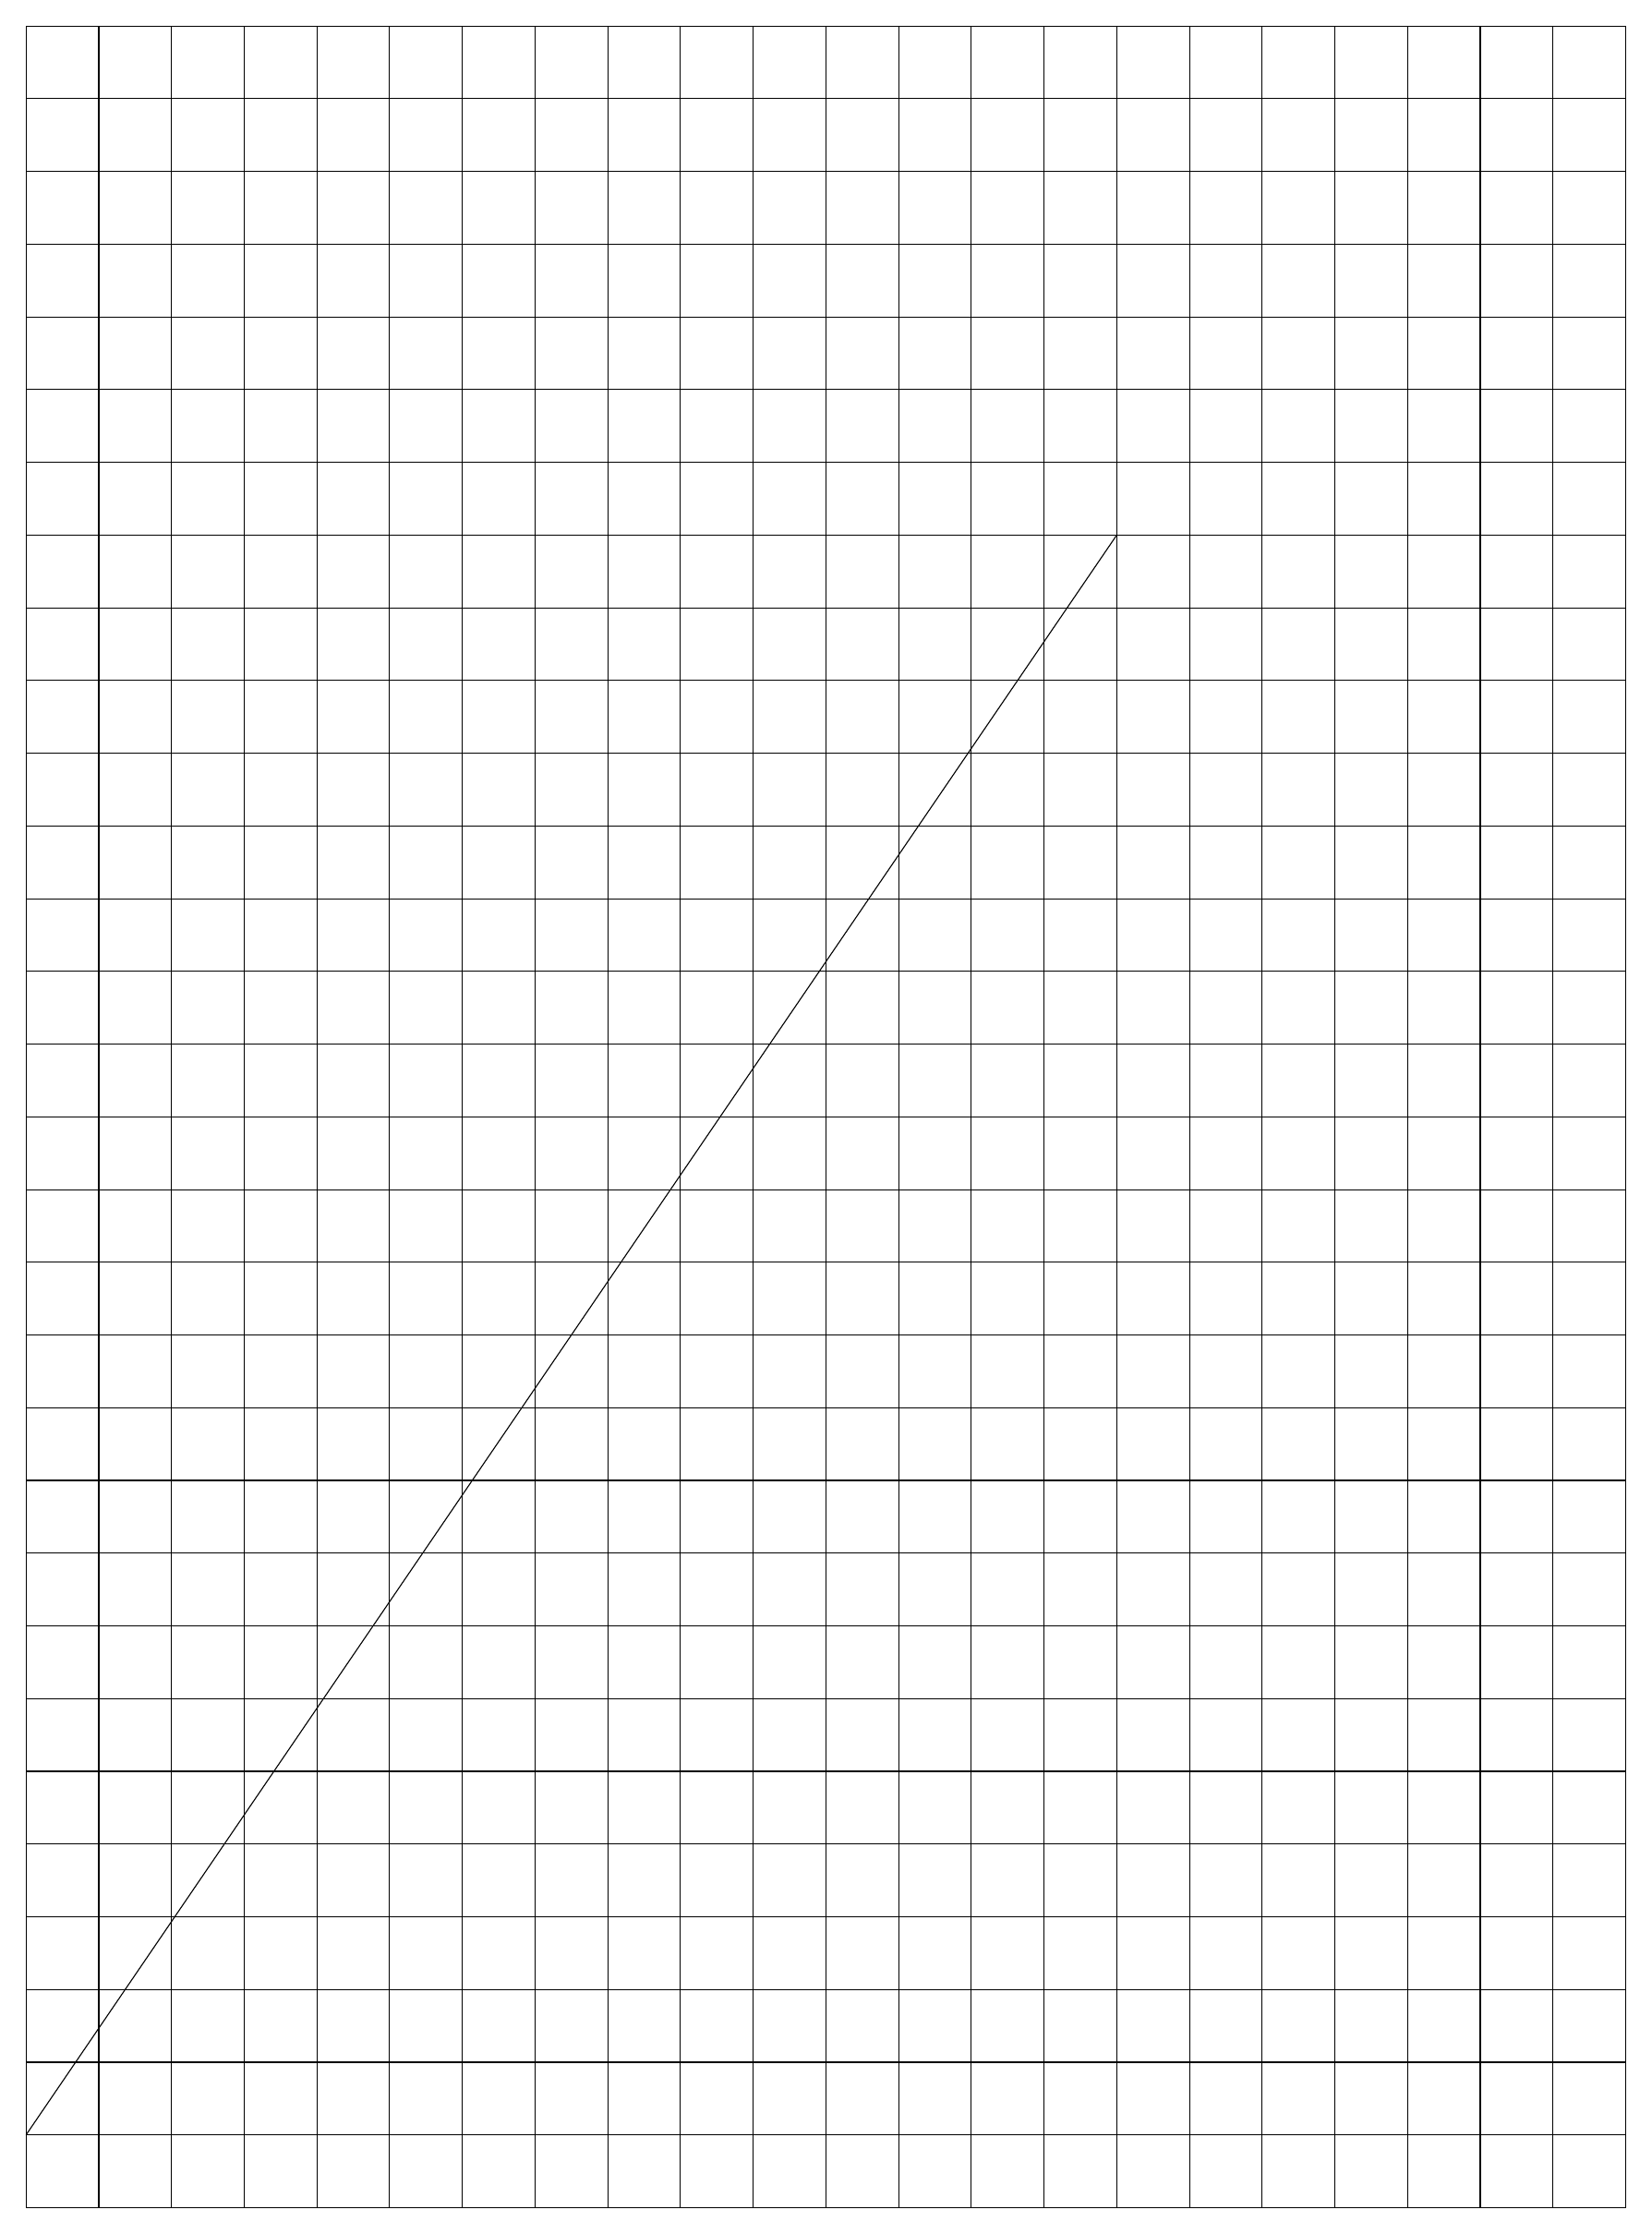
\begin{tikzpicture}
	% Grid
	\draw[](0,-3) grid (22,27);

	% Example Line
	\draw(0,-2) -- (15,20);
\end{tikzpicture}
	
	% TITLE PAGE
	\newpage
\restoregeometry		% Restore the default margins
\maketitle				% Create title
\thispagestyle{empty}	% Remove footnotes and headers
\vfill					% Push remaining text to the bottom of the page
\begin{center}
	% COVENTRY UNI LOGO
	
\includegraphics[width=5cm]{img/coventry-uni.png}\\
	
	Made with \LaTeX
\end{center}

	% TABLING (Table of Contents, Lists of Figues/Tables/Source Code)
	\newpage
\tableofcontents
\newpage
\listoffigures
\newpage
\listoftables
\newpage
\lstlistoflistings	
	
	% CONTENT
	% This .tex file structures and organizes the contents of the document allowing for a fine control of what pages come in what order.

% 6001CEM Dissertation

% PAGE EXAMPLE
\newpage
\directlua{tex.print("Hi there")}

\section{Lorem Ipsum}

\lipsum[1-5]

% CODE EXAMPLE
\newpage
\section{Rust Code}

\begin{lstlisting}[language=Rust,
	style=mystyle,
	caption={An example of Rust code.},
	label={example-rust}]
	// Your Rust code here
	fn main() {
		// Declare a mutable variable
		let mut x = 5; 
		
		// Print the initial value
		println!("The value of x is: {}", x); 
		
		// Change the value of x
		x = 6; 
		
		// Print the new value
		println!("The value of x is: {}", x); 
	}
\end{lstlisting}

% FINISHING
\newpage
	
	% GLOSSARY & BIBLIOGRAPHY
	\printglossary[type=\acronymtype]
	\newpage
	\printbibliography
\end{document}